\documentclass{article}
\usepackage{tikz}
\usetikzlibrary{positioning}
\usepackage{helvet} %font package
\usepackage{amsmath}


\tikzset{
	annulusnode/.style={
		draw=blue!70,
		fill=blue!20,
		very thick,
		minimum width=3cm,
		path picture={
			\draw[fill=white] (path picture bounding box) circle (0.7cm);
			\draw[fill=blue!50] (path picture bounding box) circle (1.5cm);
		}
	}
}



\begin{document}

\section{Drawing Point and Lines}

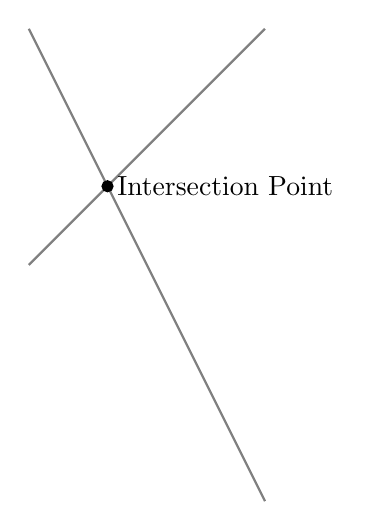
\begin{tikzpicture}

\draw[gray,thick] (-1,2) -- (2,-4);
\draw[gray,thick] (-1,-1) -- (2,2);

\filldraw[black] (0,0) circle (2pt) node[anchor=west]{Intersection Point};

\end{tikzpicture}

\section{Drawing Curves with Control Points}

\begin{tikzpicture}

\draw (-4,0) -- (4,0);
\draw (0,-4) -- (0,4);
\filldraw[black] (0,0) circle (2pt);
\draw (-2,2) .. controls (0,0) .. (2,2);
\draw (-2,-2) .. controls (-1,0) and (1,0) .. (2,-2);

\end{tikzpicture}

\section{Drawing Shapes}

\subsection{Circle, Ellipse, Arc}

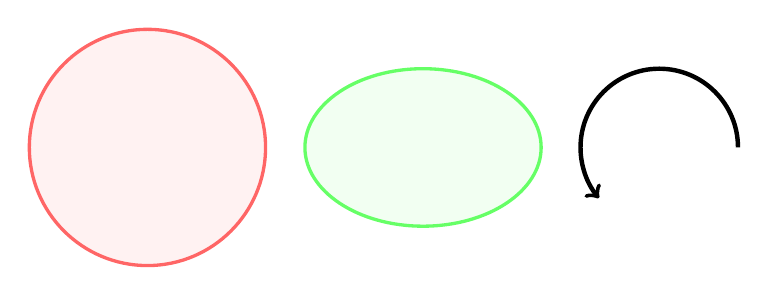
\begin{tikzpicture}
	
	
\filldraw[color=red!60, fill=red!5, very thick] (-1,0) circle (1.5);
\filldraw[color=green!60, fill=green!5, very thick] (2.5,0) ellipse (1.5 and 1);
\draw[ultra thick, ->] (6.5,0) arc (0:220:1) ;	
	
	
\end{tikzpicture}

\subsection{Rectangle, Triangle}

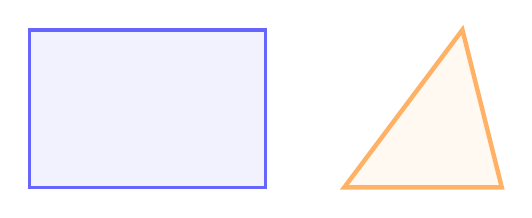
\begin{tikzpicture}
	
	
\filldraw[color=blue!60, fill=blue!5, very thick] (0,0) rectangle (3,2);
\filldraw[color=orange!60, fill=orange!5, ultra thick] (4,0) -- (6,0) -- (5.5,2) -- cycle;
	
	
\end{tikzpicture}


\section{Drawing Diagrams}

\subsection{Using Nodes}

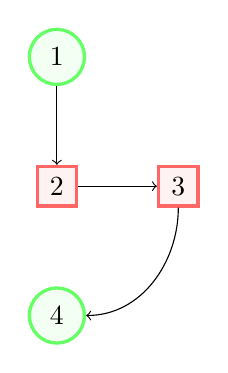
\begin{tikzpicture}[
roundnode/.style={circle, draw=green!60, fill=green!5, very thick, minimum size=7mm},
squarednode/.style={rectangle, draw=red!60, fill=red!5, very thick, minimum size=5mm},
]
	
% Nodes

\node[squarednode]      (maintopic)                              {2};
\node[roundnode]        (uppercircle)       [above=of maintopic] {1};
\node[squarednode]      (rightsquare)       [right=of maintopic] {3};
\node[roundnode]        (lowercircle)       [below=of maintopic] {4};

% Lines

\draw[->] (uppercircle.south) -- (maintopic.north);
\draw[->] (maintopic.east) -- (rightsquare.west);
\draw[->] (rightsquare.south) .. controls +(down:7mm) and +(right:7mm) .. (lowercircle.east);
	
	
\end{tikzpicture}

\subsection{Drawing Tree}


\tikzstyle{every node} = [rectangle, rounded corners, draw=blue, thick, fill=blue!10, text width=15pt, text centered]
\tikzstyle{level 1} = [sibling distance=50mm]
\tikzstyle{level 2} = [sibling distance=25mm]
\tikzstyle{level 3} = [sibling distance=12mm]

\centering
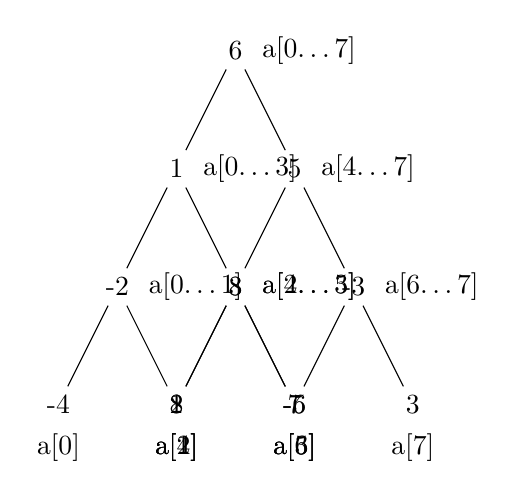
\begin{tikzpicture}
	\path
	node[label=right:\text{a[0\ldots7]}]{6}
	child{
		node[label=right:\text{a[0\ldots3]}]{1}
		child{
			node[label=right:\text{a[0\ldots1]}]{-2}
			child{
				node[label=below:\text{a[0]}]{-4}
			}
			child{
				node[label=below:\text{a[1]}]{2}
			}
		}
		child{
			node[label=right:\text{a[2\ldots3]}]{3}
			child{
				node[label=below:\text{a[2]}]{8}
			}
			child{
				node[label=below:\text{a[3]}]{-5}
			}
		}
	}
	child{
		node[label=right:\text{a[4\ldots7]}]{5}
		child{
			node[label=right:\text{a[4\ldots5]}]{8}
			child{
				node[label=below:\text{a[4]}]{1}
			}
			child{
				node[label=below:\text{a[5]}]{7}
			}
		}
		child{
			node[label=right:\text{a[6\ldots7]}]{-3}
			child{
				node[label=below:\text{a[6]}]{-6}
			}
			child{
				node[label=below:\text{a[7]}]{3}
			}
		}
	} 
	;
	
\end{tikzpicture}


\end{document}